\documentclass[11pt,a4paper]{article}
\usepackage[margin=2.4cm]{geometry}
\usepackage[T1]{fontenc}
\usepackage{mathpazo}
\renewcommand{\ttdefault}{txtt}
\usepackage{microtype}
\usepackage{amsmath,amssymb}
\usepackage{graphicx}
\usepackage{booktabs}
\usepackage{float}
\usepackage[font=small,labelfont=bf]{caption}
\usepackage{xcolor}
\usepackage{enumitem}
\usepackage{fancyhdr}
\usepackage{listings}
\usepackage{tikz}
\usetikzlibrary{positioning,arrows.meta}
\usepackage[colorlinks=true,linkcolor=black,citecolor=black,urlcolor=blue!50!black]{hyperref}

\definecolor{licit}{HTML}{2a78d6}
\definecolor{illicit}{HTML}{eb6834}
\definecolor{codebg}{HTML}{f5f5f4}
\definecolor{notebg}{HTML}{eef4fc}
\lstset{basicstyle=\ttfamily\footnotesize,backgroundcolor=\color{codebg},frame=single,rulecolor=\color{black!25},
  columns=fullflexible,keepspaces=true,showstringspaces=false,commentstyle=\itshape\color{black!55},
  keywordstyle=\bfseries,language=Python,aboveskip=6pt,belowskip=6pt,
  breaklines=true,breakatwhitespace=false,postbreak=\mbox{$\hookrightarrow$\space}}
\setlist{itemsep=3pt,topsep=4pt}
\setlength{\parskip}{4pt}
\pagestyle{fancy}\fancyhf{}
\fancyhead[R]{\small Catching Bitcoin Fraud with a Graph Convolutional Network}
\fancyfoot[C]{\thepage}
\renewcommand{\headrulewidth}{0pt}
\newcommand{\Ahat}{\hat{A}}
% a simple shaded box for "in plain words" notes
\newcommand{\plain}[1]{\par\noindent\colorbox{notebg}{\parbox{\dimexpr\linewidth-2\fboxsep}{\small\textbf{In plain words:} #1}}\par}

\title{\vspace{-1.2cm}\textbf{Catching Bitcoin Fraud with a\\ Graph Convolutional Network}\\[4pt]
\large Using a GCN on the Elliptic dataset to spot illicit transactions}
\author{\textbf{[Your name]} \\ \textcolor{red}{[roll no.]}}
\date{}

\begin{document}
\maketitle
\thispagestyle{fancy}

\section*{Summary}
Criminals use Bitcoin to move money from scams, ransomware and illegal online markets. Every Bitcoin transaction is public,
so in principle we can follow the money, but there are far too many transactions to check by hand. In this project we
train a \textbf{Graph Convolutional Network (GCN)} to look at a transaction \emph{and the transactions connected to it} and decide
whether it is \textbf{licit} (normal) or \textbf{illicit} (linked to crime).

We use the real \textbf{Elliptic dataset} of about 200,000 Bitcoin transactions. We wrote the GCN ourselves in PyTorch instead of
using a ready-made library layer, and we compared it with simpler models.

\begin{itemize}
  \item Our GCN catches a little under half of the criminal transactions in the test period, and when it raises an alarm it is
        right about 8 times out of 10.
  \item Using the connections between transactions makes the model's alarms much more trustworthy than the same model without
        them.
  \item A simple \textbf{Random Forest} model still did best overall, which matches what the creators of the dataset found.
  \item After a large illegal market was shut down, \textbf{every} model stopped working, because criminals changed their behaviour.
\end{itemize}

%=====================================================================
\section{The Problem}
%=====================================================================
Imagine you work at a bank or a crypto exchange. Thousands of Bitcoin transactions pass through every day, and a few of
them carry money from crime. You need to flag those few for an investigator to look at, without drowning the investigator
in false alarms.

The key idea of this project is simple: \textbf{a transaction is known by the company it keeps.} Money does not appear out of
nowhere. It comes from earlier transactions and flows into later ones:
\begin{center}
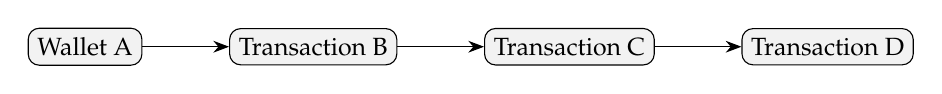
\begin{tikzpicture}[node distance=1.1cm, every node/.style={font=\small}, >={Stealth[length=2mm]}]
  \node[draw, rounded corners, fill=black!5] (w) {Wallet A};
  \node[draw, rounded corners, fill=black!5, right=of w] (b) {Transaction B};
  \node[draw, rounded corners, fill=black!5, right=of b] (c) {Transaction C};
  \node[draw, rounded corners, fill=black!5, right=of c] (d) {Transaction D};
  \draw[->] (w) -- (b); \draw[->] (b) -- (c); \draw[->] (c) -- (d);
\end{tikzpicture}
\end{center}
If B receives money from known criminal transactions, B is suspicious too, even if B looks normal on its own. A normal
machine-learning model looks at each transaction alone. A GCN also looks at its neighbours. Our plan was:
\begin{center}
\small
\textbf{Problem:} spot suspicious transactions $\;\rightarrow\;$
\textbf{Graph:} transactions and the money flowing between them $\;\rightarrow\;$
\textbf{GCN:} learns from each transaction and its neighbours $\;\rightarrow\;$
\textbf{Output:} licit or illicit
\end{center}

%=====================================================================
\section{The Dataset}
%=====================================================================
The \textbf{Elliptic dataset} \cite{weber} was released by Elliptic, a company that tracks crypto crime, together with
researchers from MIT and IBM. It is the largest public dataset of labelled Bitcoin transactions. We treat it as a graph:

\begin{itemize}
  \item \textbf{Nodes (dots):} 203,769 Bitcoin transactions.
  \item \textbf{Edges (lines):} 234,355 money flows. An edge from A to B means money that came out of A was spent in B.
  \item \textbf{Features:} each transaction has 165 numbers describing it, such as how many inputs and outputs it has, the fee,
        and the amount. 93 of these describe the transaction itself, and the other 72 summarise its direct neighbours.
        The names of the features are hidden for privacy.
  \item \textbf{Time:} every transaction belongs to one of 49 time steps, each about two weeks apart.
  \item \textbf{Labels:} 4,545 are marked \textcolor{illicit}{\textbf{illicit}}, 42,019 are marked \textcolor{licit}{\textbf{licit}},
        and 157,205 (77\%) are \textbf{unknown}. Nobody has checked those.
\end{itemize}

Figure~\ref{fig:ego} shows a real piece of the graph. About twenty illicit transactions all send money into one
transaction. This ``many-into-one'' shape is a common way to collect criminal money. You can only see it by looking at
the connections.

\begin{figure}[H]
  \centering
  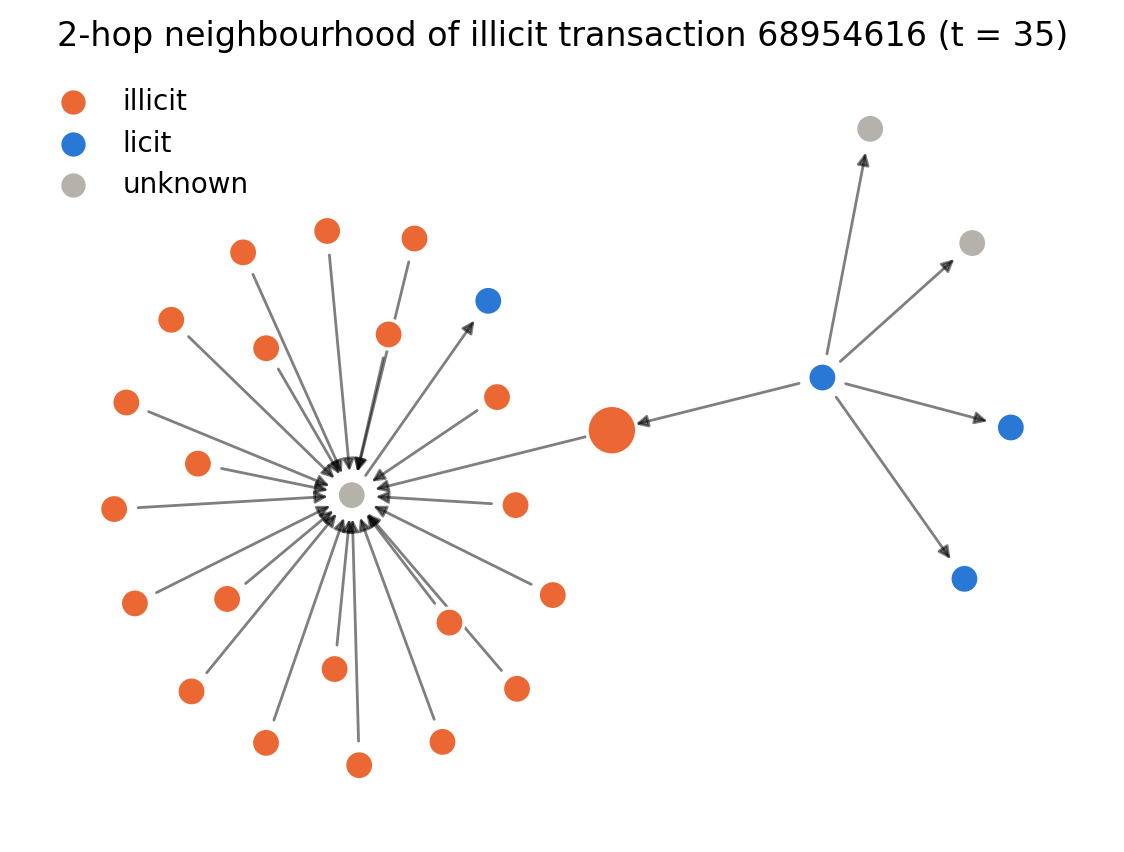
\includegraphics[width=0.58\linewidth]{figures/ego_graph.png}
  \caption{A real neighbourhood from the dataset. The big orange dot is an illicit transaction. Arrows show which way the money moved.}
  \label{fig:ego}
\end{figure}

\subsection*{Three things that make this dataset tricky}
\begin{enumerate}
  \item \textbf{Very few criminals.} Only about 1 in 10 labelled transactions is illicit. A lazy model that says ``everything is
        fine'' would be 93.5\% accurate on our test data while catching zero criminals. So \textbf{accuracy is a misleading score
        here}, and we use better ones (Section~\ref{sec:scores}).
  \item \textbf{Time matters.} We must predict the \emph{future}, not the past. So we train on time steps 1--34 and test on
        time steps 35--49, as the dataset's authors did. Transactions from different time steps are never connected, so the
        test transactions are in completely new graphs that the model has never seen.
  \item \textbf{Neighbours really do look alike.} When we checked, a neighbour of an illicit transaction was illicit 54\% of the
        time, compared with only 10\% for a random labelled transaction. This tells us the connections carry useful
        information, which is exactly what a GCN needs.
\end{enumerate}

\begin{figure}[H]
  \centering
  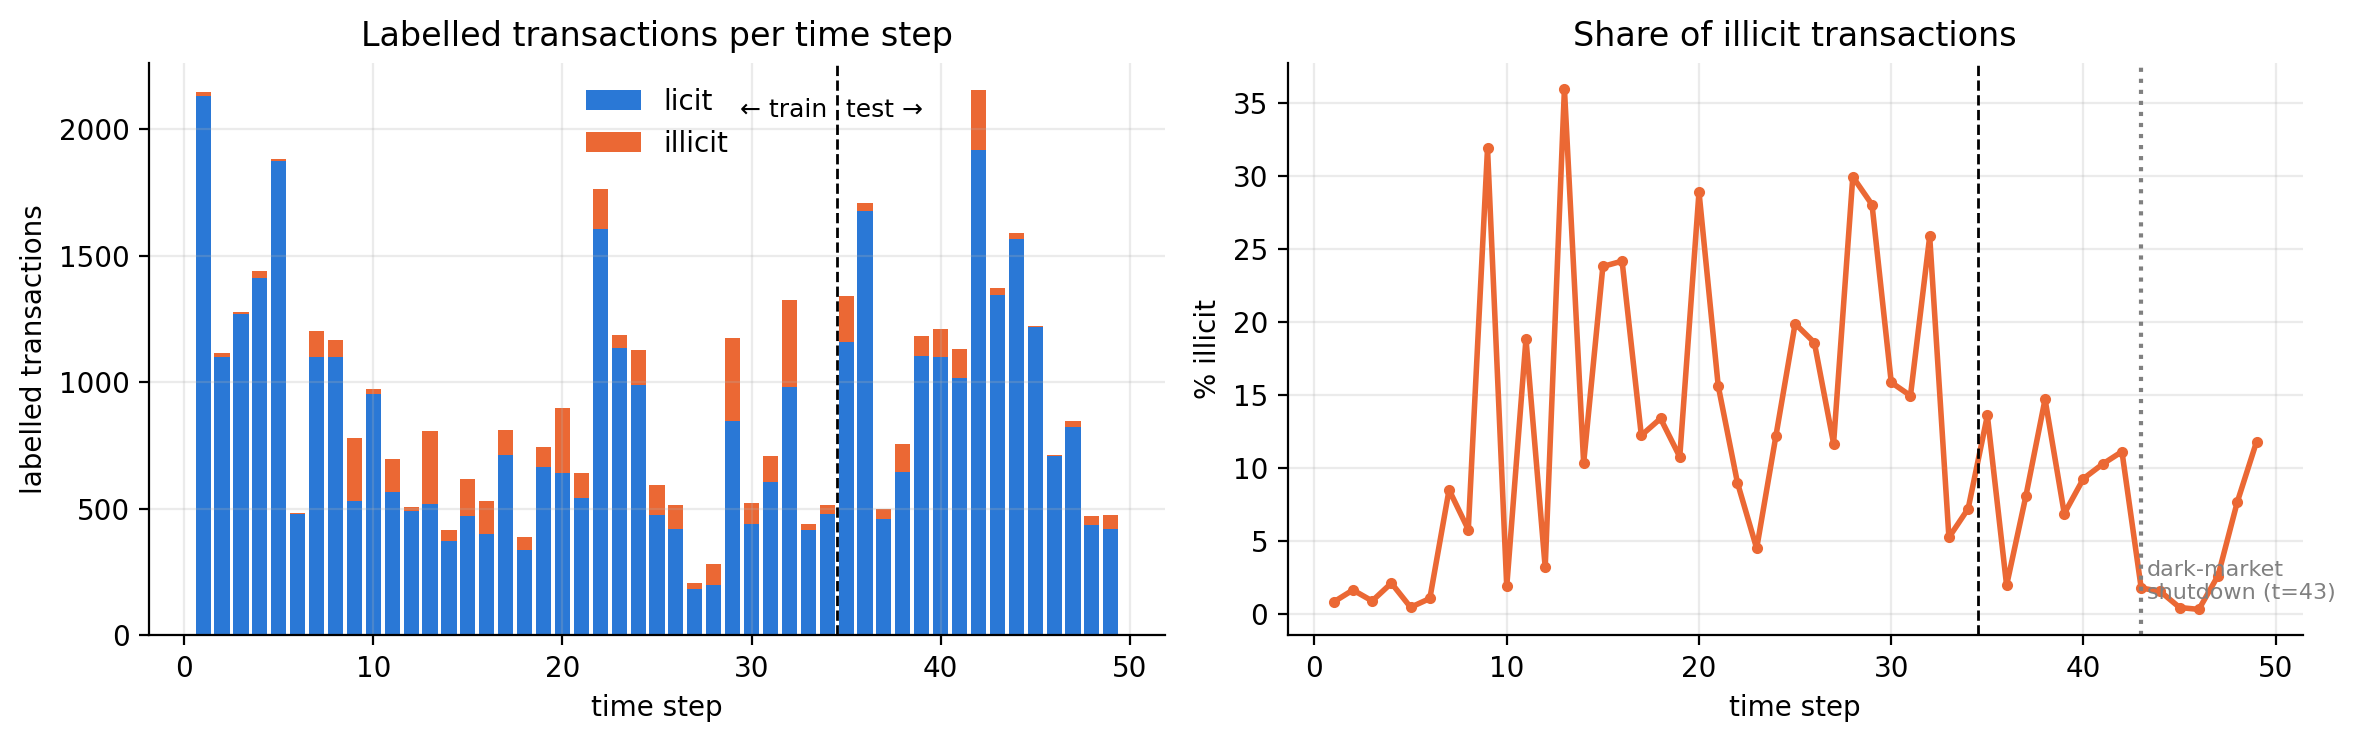
\includegraphics[width=\linewidth]{figures/dataset_timesteps.png}
  \caption{Left: labelled transactions in each time step. Right: the share that is illicit. The dashed line separates
  training (left) from testing (right).}
  \label{fig:timesteps}
\end{figure}

\begin{table}[H]
\centering\small
\begin{tabular}{ll}
\toprule
Transactions (nodes) & 203,769 \\
Money flows (edges) & 234,355 \\
Features per transaction & 165 \\
Illicit / licit / unknown & 4,545 / 42,019 / 157,205 \\
Training data (time steps 1--34) & 29,894 labelled, 3,462 of them illicit \\
Test data (time steps 35--49) & 16,670 labelled, 1,083 of them illicit \\
Average number of neighbours & 2.3 \\
\bottomrule
\end{tabular}
\caption{The dataset in numbers.}
\label{tab:data}
\end{table}

%=====================================================================
\section{What Is a GCN?}
%=====================================================================
\subsection{The idea}
A normal neural network takes a list of numbers, such as one transaction's features, and gives an answer. It cannot use
the fact that transactions are connected.

A \textbf{Graph Convolutional Network} adds one simple step: \textbf{before deciding, every node looks at its neighbours and
mixes their information with its own.} One round of mixing lets a node learn from its direct neighbours. Two rounds let it
learn from its neighbours' neighbours, two steps away. We use two rounds, called two \emph{layers}.

\plain{A GCN is like judging a person by their own behaviour \emph{and} by the people they spend time with. One layer looks at
friends; two layers also look at friends of friends.}

\subsection{Why use a GCN for this problem?}
\begin{itemize}
  \item \textbf{Fraud leaves a trail.} Criminal money is split, merged and passed along. Where the money came from and where it goes
        matters as much as the transaction itself.
  \item \textbf{Most transactions have no label.} Unlabelled transactions still pass information to their neighbours, so the
        model can use all 200,000 transactions, not just the labelled ones.
  \item \textbf{It is fast.} The model only does work along existing connections, so it handles 200,000 transactions in under a
        second on a normal laptop.
\end{itemize}

\subsection{The formula, explained step by step}
We describe the whole graph with an \textbf{adjacency matrix} $A$, a big table where $A_{ij}=1$ if transactions $i$ and $j$
are connected and 0 otherwise. The features of all transactions form a table $X$ with one row per transaction.

\textbf{Step 1: Add self-loops.} We connect every transaction to itself, $\tilde A = A + I$, so that when a node mixes in
its neighbours' information, it also keeps its own.

\textbf{Step 2: Make it fair.} Some transactions have hundreds of neighbours and most have only two. If we simply added up
neighbour information, busy nodes would get huge numbers. So we scale each connection by the number of neighbours on both
sides:
\[
  \Ahat = \tilde D^{-1/2}\,\tilde A\,\tilde D^{-1/2}
\]
which means that for two connected transactions $i$ and $j$,
\[
  \Ahat_{ij} = \frac{1}{\sqrt{(\text{neighbours of } i + 1)\times(\text{neighbours of } j + 1)}}.
\]
Here $\tilde D$ is a table that just stores how many connections each node has.

\textbf{Step 3: One GCN layer.} A layer does two things:
\[
  H_{\text{new}} = \mathrm{ReLU}\big(\,\Ahat \;\cdot\; H \;\cdot\; W\,\big)
\]
\begin{itemize}
  \item $H \cdot W$: transform each transaction's features using learned weights $W$. This is the part the model learns.
  \item $\Ahat \cdot (\dots)$: replace each transaction by a weighted average of itself and its neighbours. This is the
        ``look at the neighbours'' part.
  \item ReLU: a simple function that sets negative numbers to zero, which lets the network learn non-linear patterns.
\end{itemize}

\textbf{Step 4: Stack two layers and give an answer.}
\[
  \text{Output} = \mathrm{softmax}\Big(\Ahat \cdot \mathrm{ReLU}\big(\Ahat \cdot X \cdot W_1\big) \cdot W_2\Big)
\]
The softmax turns the final two numbers into two probabilities: ``licit'' and ``illicit''. If the illicit probability is at
least 50\%, we flag the transaction.

\plain{Each layer is ``average with your neighbours, then transform''. The only things the computer learns are the two
weight tables $W_1$ and $W_2$. The graph part, $\Ahat$, is fixed and calculated once from the connections.}

\subsection{Where does the formula come from?}
The GCN rule is not made up. It comes from \emph{graph signal processing}: just as a sound can be split into low and high
frequencies, values on a graph can be split into ``smooth'' patterns, where neighbours have similar values, and ``noisy''
patterns, where neighbours differ. Kipf and Welling \cite{kipf} reached the rule in five steps.

\textbf{Step 1: Measure how ``bumpy'' a signal is.} With degree matrix $D$, the normalised \emph{graph Laplacian} is
\[
  L = I - D^{-1/2} A D^{-1/2}, \qquad
  f^{T} L f = \tfrac12 \sum_{i,j} A_{ij}\Big(\tfrac{f_i}{\sqrt{d_i}} - \tfrac{f_j}{\sqrt{d_j}}\Big)^2 .
\]
For a value $f_i$ on every node (say, a transaction's fee), $f^T L f$ is small when connected nodes have similar values and
large when they differ.

\textbf{Step 2: Split the signal into frequencies.} $L$ is symmetric, so $L = U\Lambda U^{T}$. The eigenvectors in $U$ act like
frequencies: small eigenvalues are smooth patterns, large ones are bumpy. A \emph{graph filter} keeps some frequencies and
removes others:
\[
  g_\theta \star f = U\, g_\theta(\Lambda)\, U^{T} f .
\]
The problem: finding $U$ takes about $N^3$ operations. For $N = 203{,}769$ that is around $8\times10^{15}$, far too slow.

\textbf{Step 3: Approximate the filter with a polynomial.} Replace $g_\theta(\Lambda)$ by a polynomial in $L$:
$g_\theta \star f \approx \sum_{k=0}^{K} \theta_k L^k f$. No eigenvectors are needed, and because $(L^k)_{ij} = 0$ when $i$ and $j$
are more than $k$ steps apart, the filter only looks at nearby nodes.

\textbf{Step 4: Keep only the first step.} Use $K = 1$, approximate the largest eigenvalue by 2, and use a single
parameter $\theta$:
\[
  g_\theta \star f \approx \theta\,\big(I + D^{-1/2} A D^{-1/2}\big) f .
\]
This already means ``a node plus its neighbours''.

\textbf{Step 5: The renormalisation trick.} $I + D^{-1/2}AD^{-1/2}$ has eigenvalues between 0 and 2, so applying it again and
again makes numbers blow up or die out. Adding the self-loops \emph{before} normalising fixes this:
\[
  I + D^{-1/2}AD^{-1/2} \;\longrightarrow\; \Ahat = \tilde D^{-1/2}(A + I)\tilde D^{-1/2},
\]
whose eigenvalues lie in $(-1, 1]$. Finally the single number $\theta$ becomes a weight matrix $W$, and a non-linearity is
added, which gives exactly our layer $H_{\text{new}} = \mathrm{ReLU}(\Ahat H W)$.

\plain{A GCN layer is a cheap ``smoothing filter'' for graphs. It keeps the patterns that neighbours share and dampens the
differences between them. That is why it helps when neighbours tend to have the same label, and why too many layers make
everything look the same (Section~\ref{sec:oversmooth}).}

%=====================================================================
\section{How We Built It}
%=====================================================================
\subsection{Training the model}
\begin{enumerate}
  \item \textbf{Prepare the data.} Load the three files (features, labels, connections), scale every feature to a similar range,
        and build $\Ahat$ from the list of connections.
  \item \textbf{Make a guess.} Run all 203,769 transactions through the GCN to get an ``illicit'' probability for each one.
  \item \textbf{Measure the mistakes.} Compare the guesses with the true labels, but only for the 29,894 labelled training
        transactions.
  \item \textbf{Improve.} Adjust the weights slightly to reduce the mistakes, using the Adam optimiser.
  \item \textbf{Repeat} steps 2--4 for 200 rounds (epochs).
  \item \textbf{Test} once on time steps 35--49, which the model never saw during training.
\end{enumerate}

\textbf{Dealing with so few criminals.} Because only about 1 in 10 examples is illicit, the model could get a low error by
ignoring them. To stop this, we count a mistake on an illicit transaction as more serious than a mistake on a licit one
(weights 0.7 and 0.3, as in \cite{weber}). This is called a \emph{weighted loss}.

\begin{figure}[H]
\centering
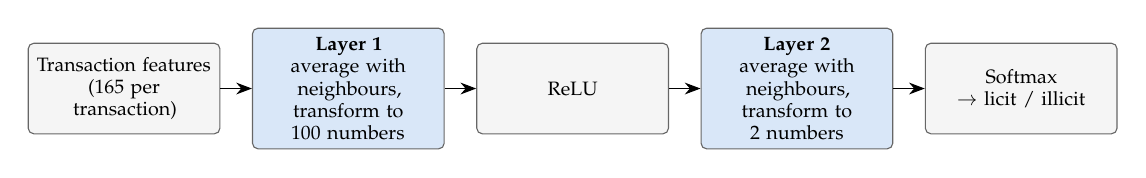
\begin{tikzpicture}[
  box/.style={draw=black!60, rounded corners=2pt, align=center, font=\scriptsize, minimum height=1.15cm, text width=2.2cm, fill=#1},
  box/.default=black!4, >={Stealth[length=2mm]}]
\node[box] (x) {Transaction features\\(165 per transaction)};
\node[box=licit!18, right=0.4cm of x] (l1) {\textbf{Layer 1}\\average with neighbours,\\transform to 100 numbers};
\node[box, right=0.4cm of l1] (relu) {ReLU};
\node[box=licit!18, right=0.4cm of relu] (l2) {\textbf{Layer 2}\\average with neighbours,\\transform to 2 numbers};
\node[box, right=0.4cm of l2] (out) {Softmax\\$\rightarrow$ licit / illicit};
\foreach \a/\b in {x/l1, l1/relu, relu/l2, l2/out} \draw[->] (\a) -- (\b);
\end{tikzpicture}
\caption{How data moves through our two-layer GCN.}
\label{fig:arch}
\end{figure}

\subsection{The code}
We wrote the GCN ourselves in PyTorch, so every line matches the formula. The two key pieces are shown here; the full model code is in the Appendix (Section~\ref{sec:code}). Building $\Ahat$:
\begin{lstlisting}
def build_norm_adj(src, dst, n):
    loops = torch.arange(n)
    row = torch.cat([src, dst, loops])     # connections in both directions + self-loops
    col = torch.cat([dst, src, loops])
    key = torch.unique(row * n + col)      # remove duplicates
    row, col = key // n, key % n
    d = torch.zeros(n).scatter_add_(0, row, torch.ones(row.numel()))   # count neighbours
    w = d[row].pow(-0.5) * d[col].pow(-0.5)                             # fair scaling
    return torch.sparse_coo_tensor(torch.stack([row, col]), w, (n, n)).coalesce()
\end{lstlisting}
One GCN layer is a single line, ``average the transformed features over the neighbours''. This is slightly simplified from the notebook, which also reuses a pre-computed $\Ahat X$ to save time:
\begin{lstlisting}
class GCNLayer(nn.Module):
    def __init__(self, in_dim, out_dim):
        super().__init__()
        self.W = nn.Parameter(torch.empty(in_dim, out_dim))
        self.b = nn.Parameter(torch.zeros(out_dim))
        nn.init.xavier_uniform_(self.W)
    def forward(self, A, H):
        return torch.sparse.mm(A, H @ self.W) + self.b      # A_hat (H W) + b
\end{lstlisting}

\textbf{A note on size.} Storing $\Ahat$ as a full table would need $203{,}769 \times 203{,}769$ numbers, about 166\,GB of
memory. But almost all of those numbers are zero, because each transaction has only a couple of neighbours. So we store
only the 672,479 non-zero entries ($2 \times 234{,}355$ connections in both directions plus 203,769 self-loops) as a
\emph{sparse} matrix, which fits easily in memory. The whole model has just \textbf{16,802} numbers to learn:
$165\times100 + 100 = 16{,}600$ in layer 1 and $100\times2 + 2 = 202$ in layer 2.

\begin{table}[H]
\centering\small
\begin{tabular}{ll}
\toprule
Size of the hidden layer & 100 \\
Optimiser & Adam, learning rate 0.01 \\
Training rounds & 200 \\
Loss & weighted, 0.7 for illicit and 0.3 for licit \\
Flag a transaction if & illicit probability $\ge$ 50\% \\
Repeated with & 5 different random starting points (seeds) \\
\bottomrule
\end{tabular}
\caption{Settings. We chose these in advance and did not tune them on the test data.}
\end{table}

\textbf{Differences from the original papers.} We follow Kipf and Welling \cite{kipf} for the optimiser (Adam, learning rate
0.01, weight decay $5\times10^{-4}$, 200 epochs) and Weber et al.\ \cite{weber} for the problem set-up (temporal split,
hidden size 100, weighted loss 0.3/0.7, no dropout). The differences are:
\begin{itemize}
  \item Kipf and Welling used 16 hidden units, dropout 0.5, weight decay on the first layer only, and stopped early based on a
        validation set. We use 100 units (as Weber et al.), no dropout, weight decay on all weights, and no early stopping,
        because a fair validation set would have to come from the past and would leave even fewer training time steps.
  \item Weber et al.\ trained for 1,000 epochs with learning rate 0.001. We use the shorter Kipf--Welling schedule
        (200 epochs, 0.01), which is faster on a laptop CPU but probably leaves our GCN slightly under-trained
        (Section~\ref{sec:published}).
  \item Our layers include a bias term $b$.
\end{itemize}

\subsection{What we compared against}
To check whether the graph really helps, we also trained:
\begin{itemize}
  \item \textbf{MLP:} exactly the same network but \emph{without} the neighbour step ($\Ahat$ replaced by ``do nothing'').
        This is the fairest comparison, because the only difference is the graph.
  \item \textbf{Skip-GCN:} a GCN with an extra shortcut, so that each transaction's own features also go straight to the
        output and are not diluted by its neighbours.
  \item \textbf{Logistic Regression} and \textbf{Random Forest:} two classic models that look at each transaction alone.
\end{itemize}
We ran every model twice: once with all 165 features, and once with only the 93 features that describe the transaction itself.

\subsection{How we score the models}
\label{sec:scores}
Since accuracy is misleading here, we use the scores a fraud team would actually care about:
\begin{itemize}
  \item \textbf{Precision:} of the transactions we flagged, how many were really illicit? Low precision means wasting
        investigators' time on false alarms.
  \item \textbf{Recall:} of all the illicit transactions, how many did we catch? Low recall means criminals slipping through.
  \item \textbf{F1 score:} one number that balances precision and recall. It is high only if both are high. This is our main score.
  \item \textbf{Ranking score (AP):} if we sort all transactions from ``most suspicious'' to ``least suspicious'', how well are the
        illicit ones pushed to the top? This does not depend on the 50\% cut-off.
\end{itemize}

\subsection{Checking that the code is right}
\label{sec:check}
Before trusting any results, we checked that the code really computes the GCN formula. We ran the notebook's own
\texttt{build\_norm\_adj} and \texttt{GCN} code on the small 5-transaction example from our maths sheet
(script \texttt{analysis/implementation\_check.py}):
\begin{enumerate}
  \item \textbf{$\Ahat$ is correct.} The matrix built by the code matches the one calculated by hand (entries such as
        $\frac12$, $\frac{1}{2\sqrt2}$, $\frac{1}{2\sqrt3}$) up to $3\times10^{-8}$, and it is symmetric.
  \item \textbf{The model computes the formula.} With random weights, the model's output and the formula
        $\Ahat\,\mathrm{ReLU}(\Ahat X W^{(0)} + b^{(0)})\,W^{(1)} + b^{(1)}$ written out with ordinary matrices differ by at most
        $1.2\times10^{-7}$. This is just computer rounding, so they are the same. The faster path that re-uses a pre-computed
        $\Ahat X$ also matches.
  \item \textbf{It reproduces the hand calculation.} With the weights of the worked example, the model gives
        $P(\text{illicit}) = 0.685$ for transaction 0 and $P(\text{licit}) = 0.746$ for transaction 4, exactly the numbers
        in the maths sheet.
\end{enumerate}
We also checked on the real data that the starting loss is sensible (Section~\ref{sec:trainbehaviour}).

%=====================================================================
\section{Results}
%=====================================================================
\subsection{Training}
\begin{figure}[H]
  \centering
  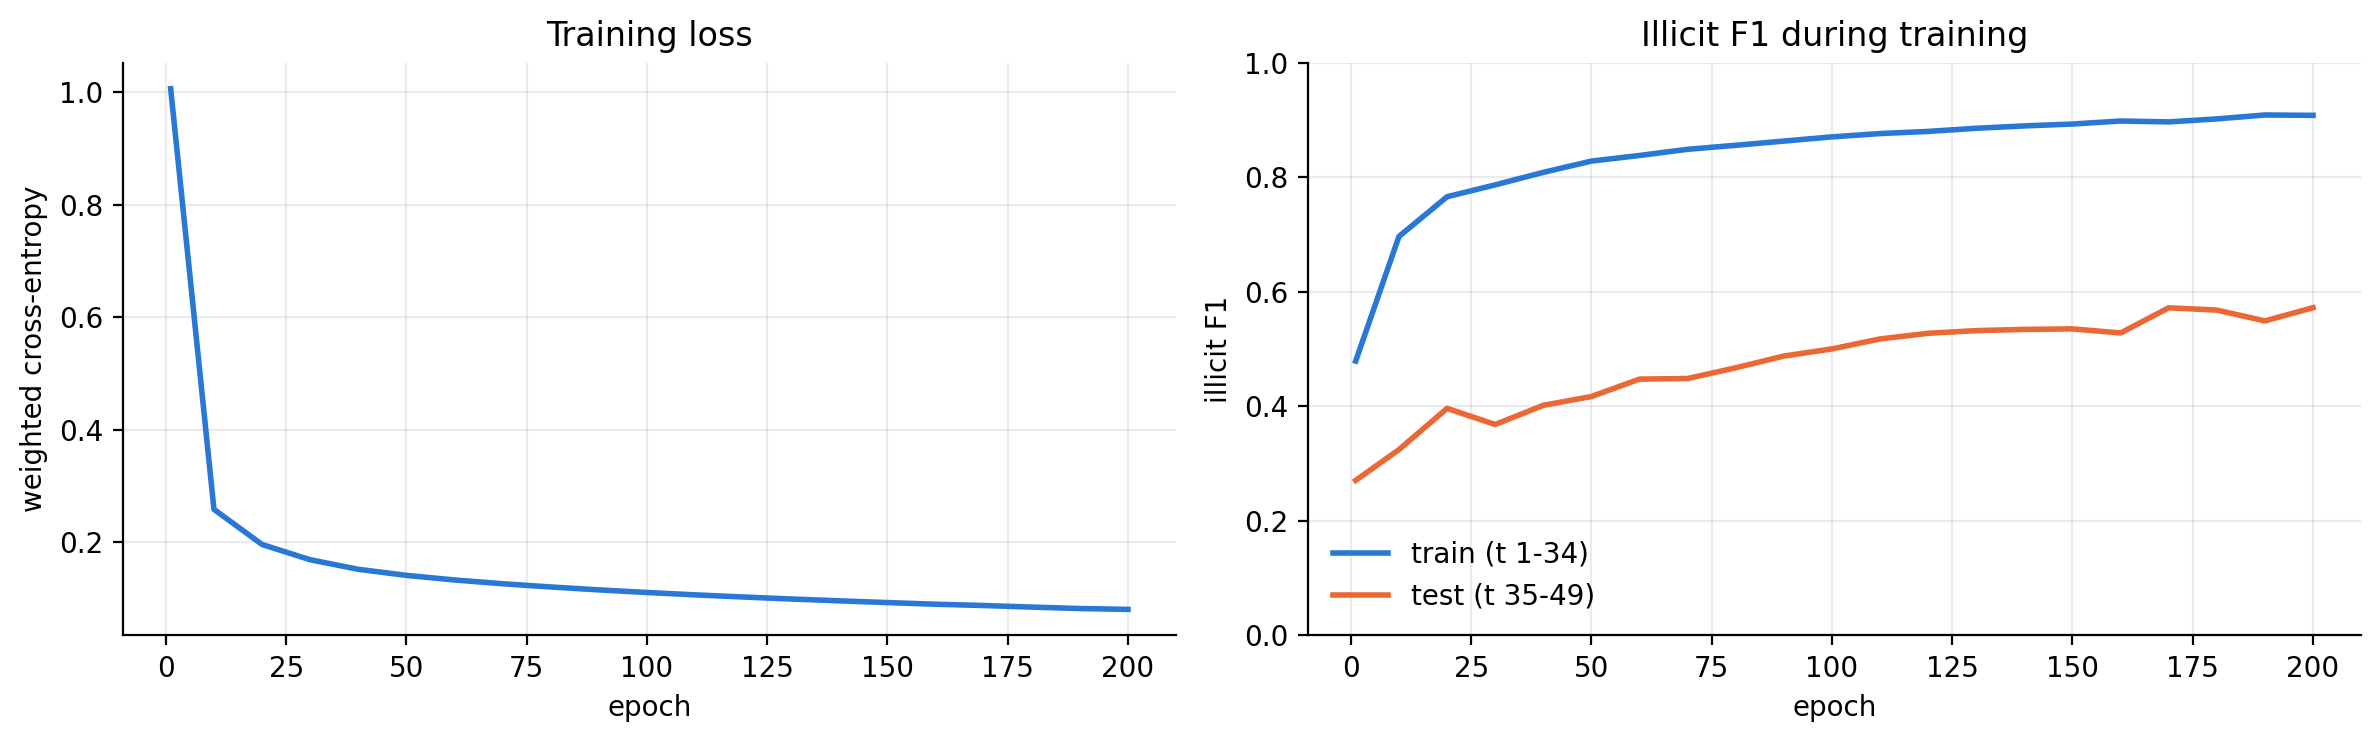
\includegraphics[width=\linewidth]{figures/training_curves.png}
  \caption{Left: the error goes down as the model learns. Right: F1 score on the training data (blue) and on the unseen
  test data (orange).}
  \label{fig:curves}
\end{figure}

\begin{table}[H]
\centering\small
\begin{tabular}{rccccc}
\toprule
Epoch & Loss & Train F1 & Test F1 & Train accuracy & Test accuracy \\
\midrule
1   & 1.0065 & 0.479 & 0.271 & 80.7\% & 82.2\% \\
20  & 0.1961 & 0.766 & 0.396 & 94.1\% & 90.8\% \\
50  & 0.1412 & 0.828 & 0.417 & 95.8\% & 92.6\% \\
100 & 0.1107 & 0.871 & 0.500 & 96.9\% & 94.5\% \\
150 & 0.0928 & 0.893 & 0.535 & 97.4\% & 95.2\% \\
200 & 0.0807 & 0.908 & 0.572 & 97.8\% & 95.5\% \\
\bottomrule
\end{tabular}
\caption{Selected rows of the training log (seed 42, all features; F1 is for the illicit class).}
\label{tab:log}
\end{table}

The error drops quickly in the first 20 rounds and then keeps falling slowly (Figure~\ref{fig:curves}, Table~\ref{tab:log}).
The F1 score on the training data reaches 0.91, while on the unseen test data it climbs to 0.57. Section~\ref{sec:general}
discusses this gap.

\begin{figure}[H]
  \centering
  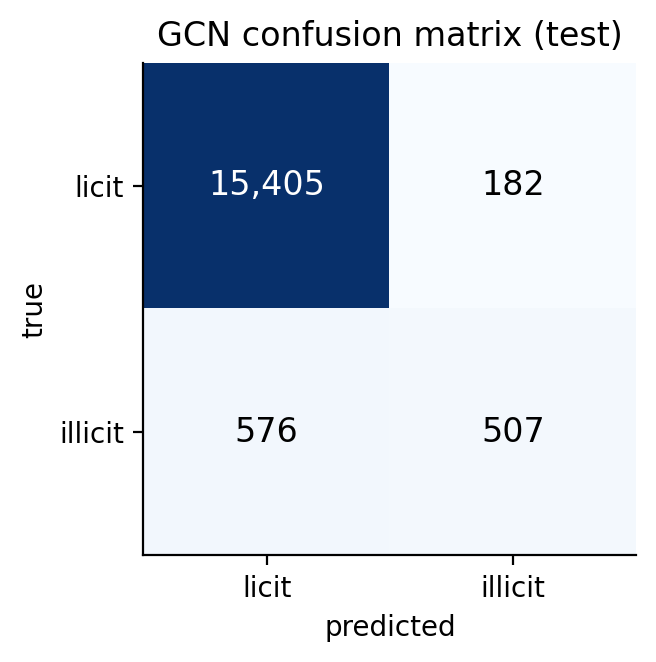
\includegraphics[width=0.36\linewidth]{figures/confusion_gcn.png}
  \caption{What the GCN got right and wrong on the 16,670 test transactions.}
  \label{fig:cm}
\end{figure}
Figure~\ref{fig:cm} shows the GCN's decisions on the test data. It flagged 689 transactions, and 507 of them really were
illicit, so \textbf{74\% of its alarms were correct}. It caught 507 of the 1,083 illicit transactions (47\%) and missed the rest.

\subsection{Comparing all the models}
\begin{table}[H]
\centering\small
\begin{tabular}{llcccc}
\toprule
Features used & Model & Precision & Recall & \textbf{F1 score} & Ranking (AP) \\
\midrule
All 165 & Logistic Regression & 0.31 & 0.68 & 0.43 & 0.32 \\
        & MLP (no graph)      & 0.56 & 0.54 & 0.55 & 0.44 \\
        & \textbf{GCN (ours)} & \textbf{0.79} & 0.44 & 0.56 & \textbf{0.60} \\
        & Skip-GCN            & 0.76 & 0.47 & 0.58 & 0.60 \\
        & Random Forest       & 0.92 & 0.72 & \textbf{0.81} & 0.78 \\
\midrule
Own 93 only & Logistic Regression & 0.39 & 0.71 & 0.51 & 0.30 \\
        & MLP (no graph)      & 0.45 & 0.75 & 0.56 & 0.52 \\
        & \textbf{GCN (ours)} & 0.43 & 0.60 & 0.50 & 0.53 \\
        & Skip-GCN            & 0.39 & 0.62 & 0.48 & 0.49 \\
        & Random Forest       & 0.85 & 0.71 & \textbf{0.77} & 0.77 \\
\bottomrule
\end{tabular}
\caption{Test results, averaged over 5 runs (higher is better for every column).}
\label{tab:final}
\end{table}

\begin{figure}[H]
  \centering
  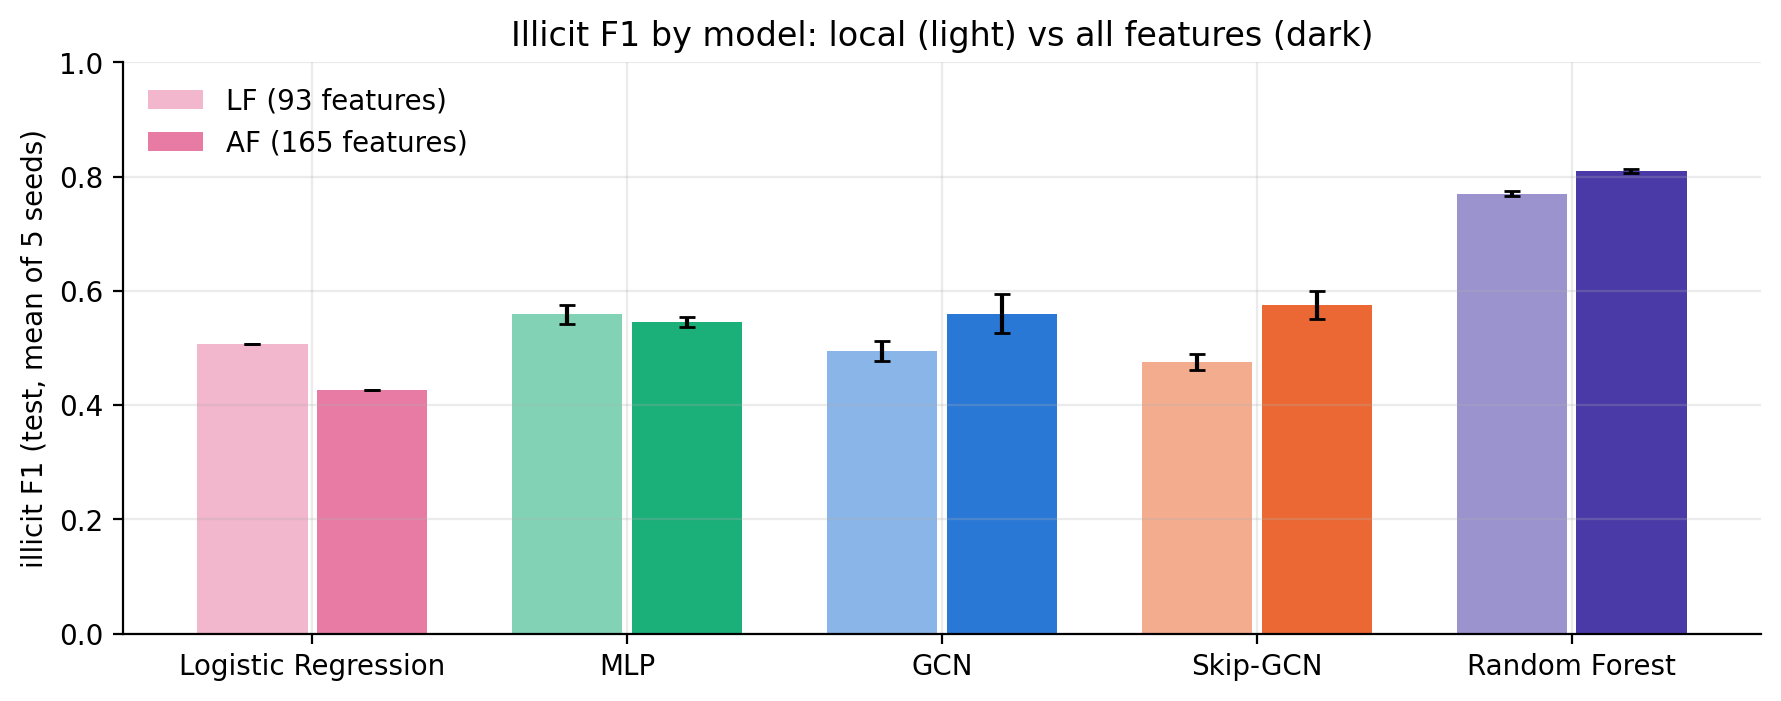
\includegraphics[width=0.85\linewidth]{figures/model_comparison.png}
  \caption{F1 score of each model. Light bars use only a transaction's own 93 features; dark bars use all 165.}
  \label{fig:comparison}
\end{figure}

\subsection{Results over time}
\begin{figure}[H]
  \centering
  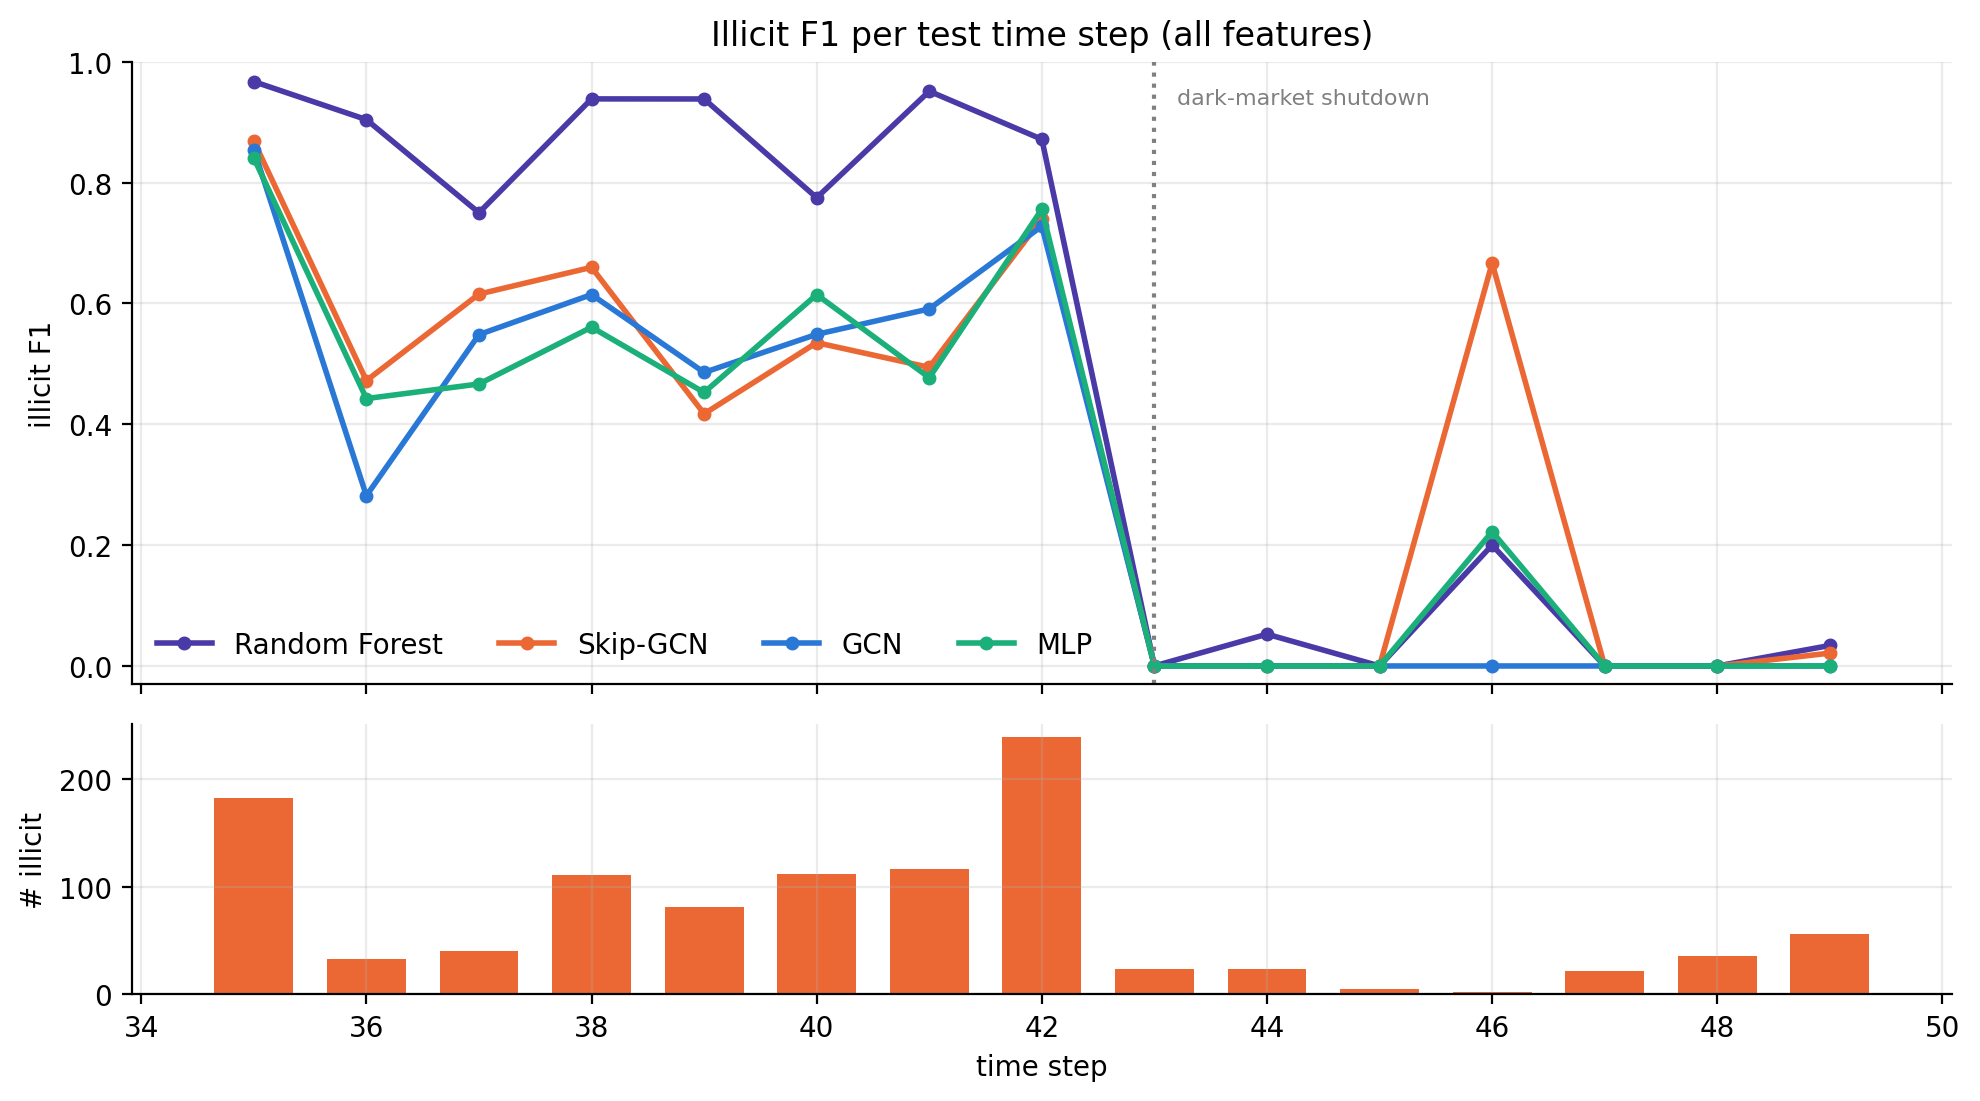
\includegraphics[width=0.9\linewidth]{figures/f1_per_timestep.png}
  \caption{F1 score of each model in each test time step (top), and how many illicit transactions each time step had (bottom).}
  \label{fig:perstep}
\end{figure}

\subsection{Does adding more layers help?}
\begin{figure}[H]
  \centering
  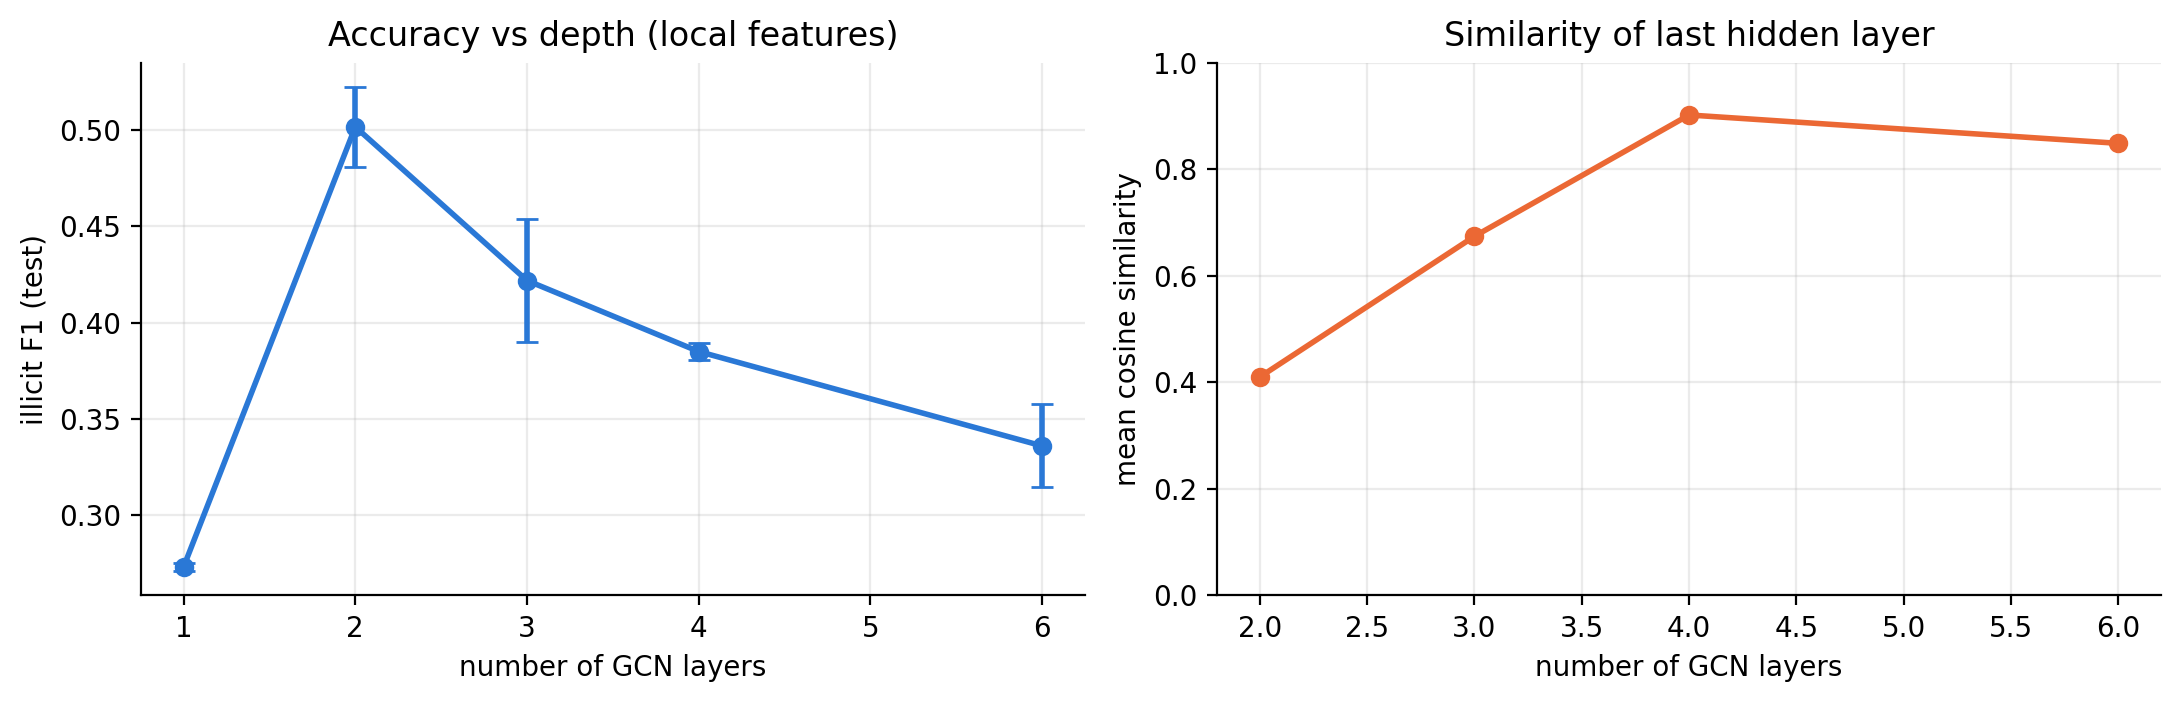
\includegraphics[width=0.9\linewidth]{figures/depth.png}
  \caption{Left: F1 score as we add more GCN layers. Right: how similar the transactions look to each other inside the model
  (1 = all identical).}
  \label{fig:depth}
\end{figure}

\subsection{Over-smoothing without training}
To see what the averaging step does on its own, we took random features $H_0$ (16 numbers per transaction) and applied
$\Ahat$ again and again, with no weights and no ReLU: $H_k = \Ahat^k H_0$. After each step we measured how similar 1,000
random transactions are to each other (mean cosine similarity: 0 = unrelated, 1 = identical), both across the whole graph and
inside its largest connected piece, time step 1 with 7,880 transactions (script \texttt{analysis/oversmoothing\_untrained.py}).

\begin{table}[H]
\centering\small
\setlength{\tabcolsep}{3.6pt}
\begin{tabular}{lccccccccccc}
\toprule
Steps $k$ & 1 & 2 & 4 & 8 & 16 & 32 & 64 & 128 & 256 & 512 & 1024 \\
\midrule
Largest component & 0.000 & 0.000 & 0.000 & 0.003 & 0.009 & 0.030 & 0.092 & 0.256 & 0.507 & 0.710 & 0.855 \\
All nodes         & 0.000 & $-$0.001 & $-$0.001 & $-$0.001 & 0.000 & 0.000 & 0.002 & 0.005 & 0.010 & 0.014 & 0.016 \\
\bottomrule
\end{tabular}
\caption{Similarity of transactions after $k$ averaging steps, with no training.}
\label{tab:untrained}
\end{table}

\begin{figure}[H]
  \centering
  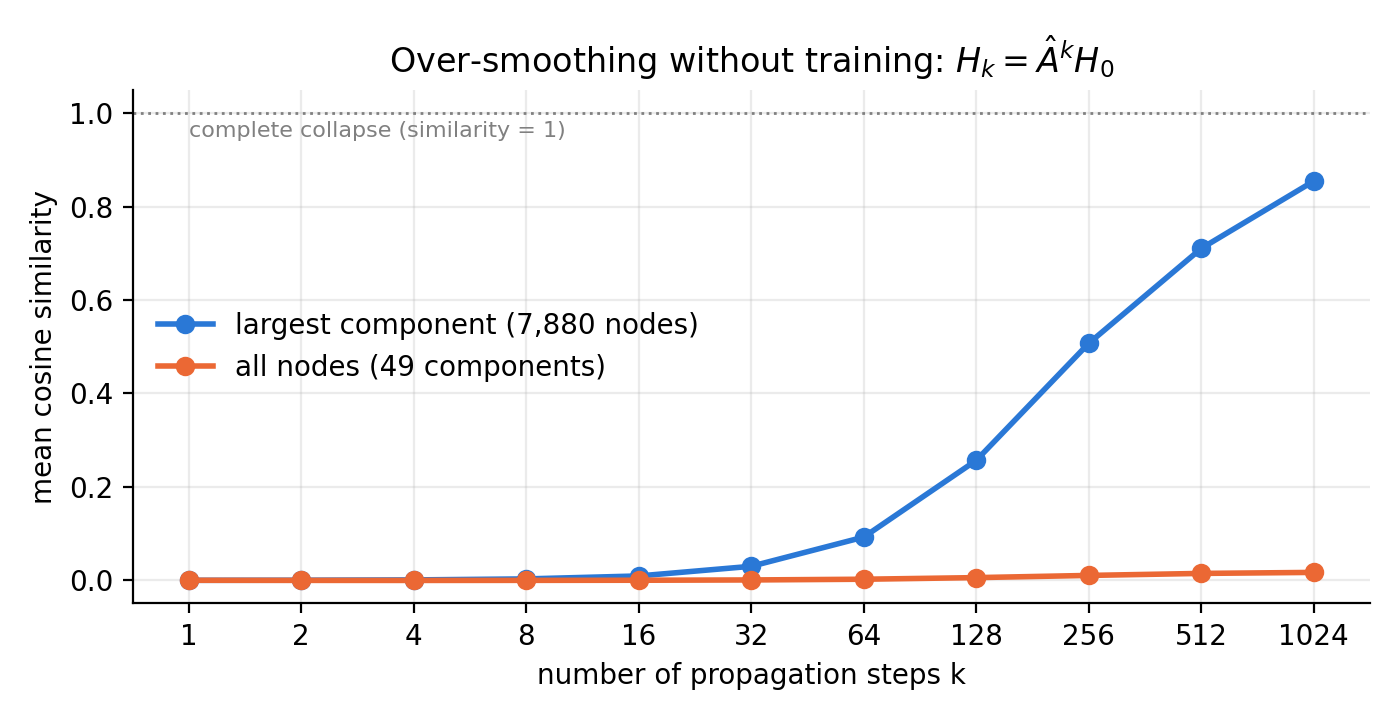
\includegraphics[width=0.78\linewidth]{figures/oversmoothing_untrained.png}
  \caption{The same numbers as a graph. Inside one connected piece, the transactions slowly become identical.}
  \label{fig:untrained}
\end{figure}

%=====================================================================
\section{What We Learned}
%=====================================================================
\subsection{How training behaved}
\label{sec:trainbehaviour}
A model that has learned nothing and gives 50/50 answers would have a loss of $\ln 2 \approx 0.693$. Our first loss is 1.007,
a little higher, because the random starting weights make some confident wrong guesses. It is in the right range, which is
a useful sign that the loss is implemented correctly. Training then has two phases:
\begin{itemize}
  \item \textbf{Fast learning (epochs 1--20).} The loss falls from 1.01 to 0.20 and training F1 jumps from 0.48 to 0.77.
  \item \textbf{Slow improvement (epochs 20--200).} The loss keeps falling slowly to 0.08, and test F1 keeps rising,
        from 0.40 to 0.57. It is still rising at epoch 200, so longer training would probably help a little.
\end{itemize}
The curves are smooth, with no jitter, because we use no dropout.

\subsection{The gap between training and test}
\label{sec:general}
Training F1 reaches 0.91 but test F1 only 0.57. The usual suspect, memorising the training data, is unlikely here: the model
has only 16,802 weights for 29,894 labelled training transactions (about 0.6 weights per example). The main cause is
\textbf{time}. The test transactions come from later time steps and from completely new graphs, and criminal behaviour keeps
changing. Figure~\ref{fig:perstep} shows this directly: on the first test step (35) the GCN scores 0.86, but after the
market shutdown at step 43 it falls to almost zero.

\textbf{How reliable are the numbers?} The test period contains 16,670 labelled transactions but only 1,083 illicit ones,
so the scores carry some noise. For recall $p = 0.468$ measured on 1,083 illicit transactions, the standard error is
$\sqrt{p(1-p)/1083} \approx 0.015$, and for precision it is $\sqrt{0.736 \times 0.264 / 689} \approx 0.017$. Repeating the
training with 5 different seeds gives a GCN F1 of $0.560 \pm 0.034$. Differences between models smaller than about
0.03--0.04 should therefore not be over-interpreted.

\subsection{The graph makes alarms more trustworthy}
The fairest test of the graph is GCN versus MLP, because they are the same network and the only difference is whether it
looks at neighbours. With all features:
\begin{itemize}
  \item \textbf{Precision rose from 56\% to 79\%}, so far fewer false alarms.
  \item The \textbf{ranking score rose from 0.44 to 0.60}, so illicit transactions are pushed much closer to the top of the list.
  \item But \textbf{recall dropped} from 54\% to 44\%, so the F1 score only improved a little (0.55 to 0.56).
\end{itemize}
In other words, looking at neighbours made the model more careful and more accurate when it raised an alarm, but also a bit more
hesitant to raise one. In practice, a bank could lower the 50\% cut-off to catch more criminals while keeping fairly good precision.

\subsection{But the graph is not magic}
When we gave the models only each transaction's own 93 features, the GCN did \emph{not} beat the MLP on F1 (0.50 versus 0.56).
The original researchers saw the same thing \cite{weber}. We think there are three reasons:
\begin{itemize}
  \item \textbf{Too much averaging.} Most transactions have only about two neighbours, so when a node averages with them,
        half or more of its own information is replaced by theirs. Since 77\% of transactions are unlabelled, much of what gets
        mixed in carries no clear signal.
  \item \textbf{Criminal transactions often touch normal ones.} Only about half of an illicit transaction's labelled neighbours
        are illicit, so averaging can water down exactly the rare signal we want to find.
  \item \textbf{The future looks different.} The test graphs are new, and the connection patterns learned from the past
        carry over less well than simple per-transaction facts.
\end{itemize}

\subsection{The simple model won}
The Random Forest scored best (F1 0.81), just as in the original study. Random Forests are very good at tables of mixed
numbers such as amounts, fees and counts, and they can learn sharp rules like ``fee above X and more than Y outputs''. This is a
useful reminder that a fancier model is not always better. The best choice depends on the data.

\subsection{How do we compare with the original paper?}
\label{sec:published}
\begin{table}[H]
\centering\small
\begin{tabular}{llcc}
\toprule
Features & Model & Our F1 (5 seeds) & Weber et al.\ \cite{weber} \\
\midrule
All 165 & Logistic Regression & 0.43 & 0.48 \\
        & MLP                 & 0.55 & 0.65 \\
        & GCN                 & 0.56 & 0.63 \\
        & Skip-GCN            & 0.58 & 0.71 \\
        & Random Forest       & \textbf{0.81} & \textbf{0.79} \\
\midrule
Own 93 only & Logistic Regression & 0.51 & 0.46 \\
        & MLP                 & 0.56 & 0.65 \\
        & Random Forest       & \textbf{0.77} & \textbf{0.69} \\
\bottomrule
\end{tabular}
\caption{Illicit F1 on the same temporal split: our results next to the published ones.}
\label{tab:published}
\end{table}
\begin{itemize}
  \item \textbf{The big picture is the same.} In both studies the Random Forest is clearly the best model, Skip-GCN beats the
        plain GCN, and the plain GCN does \emph{not} beat the MLP.
  \item \textbf{Our Random Forest is slightly better} (0.81 versus 0.79), and our Logistic Regression is close.
  \item \textbf{Our neural models are 0.07--0.13 lower.} The most likely reason is training: Weber et al.\ trained for
        1,000 epochs (we used 200) and may have tuned their networks, while we fixed standard settings in advance. Our test
        F1 was still rising at epoch 200 (Table~\ref{tab:log}). Their exact code and settings were not published, so this is a
        reference point rather than an exact replication.
\end{itemize}

\subsection{Every model failed when criminals changed their behaviour}
Figure~\ref{fig:perstep} may be the most important result. Up to time step 42, all models work reasonably well. At time step 43
a big illegal online market was shut down, and from that point \textbf{every model's F1 score falls to almost zero}. (The jump at
time step 46 is just luck: that time step had only 2 illicit transactions.)

Criminals simply started doing things differently, and models trained on old patterns could not recognise the new ones. This is
called \textbf{concept drift}. It means a real fraud-detection system must be retrained regularly with fresh data. No model
choice can fix this on its own.

\subsection{Two layers is the sweet spot}
\label{sec:oversmooth}
Figure~\ref{fig:depth} shows what happens with more layers. One layer is too simple (F1 0.27), two layers work best (0.50), and
after that the score keeps falling (0.42, 0.39, 0.34). At the same time, the transactions start to look more and more alike
inside the model: their similarity rises from 0.41 to 0.90.

This is called \textbf{over-smoothing} \cite{li}. Every layer averages each node with its neighbours. Do this many times and everything
in the same area is averaged into the same grey mush, so illicit and licit transactions can no longer be told apart. That is
why GCNs are usually kept to two or three layers.

\plain{Averaging with your friends once gives you useful context. Averaging with friends of friends of friends of friends
makes everyone in town look the same.}

\textbf{Why it happens (the maths).} $\Ahat$ is symmetric, so it can be written using its eigenvalues $\mu_i$ and
eigenvectors $u_i$: $\Ahat = \sum_i \mu_i u_i u_i^{T}$. On a connected graph the largest eigenvalue is exactly
$\mu_1 = 1$, with eigenvector $\pi \propto \tilde D^{1/2}\mathbf 1$ (one can check $\Ahat\pi = \pi$), and every other eigenvalue
has $|\mu_i| < 1$. Applying $\Ahat$ $k$ times multiplies each part by $\mu_i^k$:
\[
  \Ahat^{k} H = \pi\pi^{T} H + \sum_{i\ge 2} \mu_i^{k}\, u_i u_i^{T} H \;\longrightarrow\; \pi\pi^{T} H
  \qquad (k \to \infty),
\]
because $\mu_i^k \to 0$ for every $i \ge 2$. In the limit, every row, which means every transaction, becomes a multiple of
the same vector $\pi^T H$, so all transactions point in the same direction \cite{li,oono}. How fast this happens depends on
the second-largest eigenvalue $\lambda_2 = \max_{i\ge2}|\mu_i|$: the leftover differences shrink like $\lambda_2^{\,k}$.

\textbf{What we observe without training} (Table~\ref{tab:untrained}, Figure~\ref{fig:untrained}):
\begin{itemize}
  \item Inside the largest connected piece (7,880 transactions), similarity climbs from 0.00 to 0.26 after 128 steps and
        0.85 after 1,024 steps, heading towards 1 as the maths predicts.
  \item It is slow because $\lambda_2 = 0.99958$ on this piece, very close to 1. Bitcoin transaction graphs are long, thin chains
        (on average only 2.3 neighbours), so information spreads slowly.
  \item Across the whole graph, similarity stays near 0 (0.016 after 1,024 steps). The graph is made of 49 separate pieces, one
        per time step, and each piece smooths towards its \emph{own} direction.
\end{itemize}
In the \emph{trained} models (Figure~\ref{fig:depth}), similarity rose much faster, to 0.90 after only 4 layers. The learned
weights and ReLU also squash and mix the features at every layer, so in practice a GCN can over-smooth after just a few layers
even on a graph where pure averaging is slow. That matches the drop in F1 we measured after 2 layers.

%=====================================================================
\section{Limitations}
%=====================================================================
\textbf{Limitations of our experiment}
\begin{itemize}
  \item \textbf{We did not tune the settings.} We used standard values to keep the test fair, and we had no validation period
        to spare. With tuning and longer training, the GCN would probably score higher; the original paper reached 0.63.
  \item \textbf{Only 5 runs} (2 for the depth study), and the training curves and log come from a single seed. Differences of
        about 0.03 in F1 between the neural models could be down to chance (Section~\ref{sec:general}).
  \item \textbf{The test curve is only plotted.} It was recorded every 10 epochs for the figures and was not used to choose
        anything; the reported model is always the one after the last epoch.
  \item \textbf{Few illicit examples after the shutdown.} Time steps 43--49 contain only a handful of illicit transactions
        (2 at step 46), so per-step scores there are very noisy.
  \item \textbf{A fixed 50\% cut-off.} It is not the best cut-off for F1 for any model; the ranking score (AP) is reported to make
        up for this.
  \item \textbf{The untrained over-smoothing test uses random features and cosine similarity,} which ignores the size of the
        vectors. It shows what averaging does, not exactly what happens inside a trained model.
\end{itemize}

\textbf{Limitations of the vanilla GCN itself}, and known fixes:
\begin{itemize}
  \item \textbf{Over-smoothing limits depth.} Fixes: skip or residual connections (like our Skip-GCN), JK-Net, APPNP, DropEdge.
  \item \textbf{All neighbours count the same}, weighted only by degree. Fix: Graph Attention Networks (GAT), which learn which
        neighbours matter more.
  \item \textbf{It ignores the direction of money flow.} We treated ``A pays B'' the same as ``B pays A''. Fix: directed graph
        networks that treat incoming and outgoing money separately.
  \item \textbf{It assumes neighbours are alike (homophily).} Only about half of an illicit transaction's labelled neighbours are
        illicit, so averaging can hide the rare signal.
  \item \textbf{It is static.} It cannot adapt when criminal behaviour changes (concept drift). Fixes: regular retraining,
        temporal models such as EvolveGCN.
  \item \textbf{It needs the whole graph in memory} for every training step (full-batch). Fixes: neighbour sampling
        (GraphSAGE) or training on clusters (Cluster-GCN).
\end{itemize}

%=====================================================================
\section{Conclusion}
%=====================================================================
We built a Graph Convolutional Network from scratch and used it on a real problem: finding criminal Bitcoin transactions among
more than 200,000. The GCN uses a simple idea, that a transaction should be judged together with the transactions it is
connected to.

Looking at neighbours made the model's alarms much more reliable (precision 79\% versus 56\% without the graph), and we saw
first-hand why GCNs are kept shallow. We also found the limits of the approach. A well-tuned Random Forest still won, and
every model broke down when criminals changed their behaviour after a market shutdown. The main lesson is that graphs are a
powerful extra source of information for fraud detection, but in the real world keeping the model up to date matters as much
as choosing it.

\begin{thebibliography}{9}\small
\bibitem{kipf} T.~N.~Kipf and M.~Welling. Semi-Supervised Classification with Graph Convolutional Networks. \emph{ICLR}, 2017.
\bibitem{weber} M.~Weber, G.~Domeniconi, J.~Chen, D.~K.~I.~Weidele, C.~Bellei, T.~Robinson and C.~E.~Leiserson. Anti-Money Laundering in
Bitcoin: Experimenting with Graph Convolutional Networks for Financial Forensics. \emph{KDD Workshop on Anomaly Detection in Finance}, 2019.
\bibitem{li} Q.~Li, Z.~Han and X.-M.~Wu. Deeper Insights into Graph Convolutional Networks for Semi-Supervised Learning. \emph{AAAI}, 2018.
\bibitem{oono} K.~Oono and T.~Suzuki. Graph Neural Networks Exponentially Lose Expressive Power for Node Classification. \emph{ICLR}, 2020.
\end{thebibliography}

\clearpage
%=====================================================================
\section{Appendix: Model Code}\label{sec:code}
%=====================================================================
This appendix lists the code of the model exactly as it appears in the notebook \texttt{gcn\_elliptic.ipynb}
(cells that only draw figures or print statistics are left out). Everything is plain PyTorch; no pre-built graph layer is used.

\subsection*{A.1 \ Setup and imports}
Libraries, random seed and plot colours.
\begin{lstlisting}
import os, time, random
import numpy as np
import pandas as pd
import scipy.sparse as sp
from scipy.sparse.csgraph import connected_components
import torch
import torch.nn as nn
import torch.nn.functional as F
import matplotlib.pyplot as plt
import networkx as nx
from sklearn.linear_model import LogisticRegression
from sklearn.ensemble import RandomForestClassifier
from sklearn.metrics import (precision_score, recall_score, f1_score, accuracy_score,
                             confusion_matrix, average_precision_score)

def set_seed(seed):
    random.seed(seed); np.random.seed(seed); torch.manual_seed(seed)

set_seed(42)
torch.set_num_threads(os.cpu_count())
os.makedirs("figures", exist_ok=True)

# colours used in every figure
C_LICIT, C_ILLICIT, C_UNKNOWN = "#2a78d6", "#eb6834", "#b4b2ab"
C_MODEL = {"GCN": "#2a78d6", "Skip-GCN": "#eb6834", "MLP": "#1baf7a", "Random Forest": "#4a3aa7",
           "Logistic Regression": "#e87ba4"}
plt.rcParams.update({"figure.dpi": 110, "axes.spines.top": False, "axes.spines.right": False,
                     "axes.grid": True, "grid.alpha": 0.25, "font.size": 10})

print("PyTorch", torch.__version__, "| NumPy", np.__version__, "| pandas", pd.__version__)
\end{lstlisting}

\subsection*{A.2 \ Loading the Elliptic dataset}
Reads the three CSV files (features, labels, edges). If they are missing, PyTorch Geometric is used only to download them.
\begin{lstlisting}
FILES = ["elliptic_txs_features.csv", "elliptic_txs_classes.csv", "elliptic_txs_edgelist.csv"]

def locate_raw_files(data_dir="data/elliptic_bitcoin_dataset"):
    if all(os.path.exists(os.path.join(data_dir, f)) for f in FILES):
        return data_dir
    from torch_geometric.datasets import EllipticBitcoinDataset   # downloader only
    EllipticBitcoinDataset("data/pyg_elliptic")
    return "data/pyg_elliptic/raw"

raw_dir = locate_raw_files()
t0 = time.time()
feat_df  = pd.read_csv(os.path.join(raw_dir, FILES[0]), header=None)
class_df = pd.read_csv(os.path.join(raw_dir, FILES[1]))
edge_df  = pd.read_csv(os.path.join(raw_dir, FILES[2]))
print(f"loaded from {raw_dir} in {time.time()-t0:.1f}s")
print("features:", feat_df.shape, "| classes:", class_df.shape, "| edges:", edge_df.shape)
\end{lstlisting}

\subsection*{A.3 \ Features, labels and edges}
Turns the CSV files into a feature matrix, a label vector ($-1$ unknown, 0 licit, 1 illicit) and the list of money flows.
\begin{lstlisting}
tx_ids    = feat_df[0].values
time_step = feat_df[1].values.astype(int)
X_all     = feat_df.iloc[:, 2:].values.astype(np.float32)        # 165 features
LOCAL, AGG = slice(0, 93), slice(93, 165)                         # 93 local + 72 aggregated

N = len(tx_ids)
pos = pd.Series(np.arange(N), index=tx_ids)                        # txId -> row index

label_str = class_df.set_index("txId").loc[tx_ids, "class"].astype(str).values
y_np = np.full(N, -1, dtype=np.int64)          # -1 unknown, 0 licit, 1 illicit
y_np[label_str == "2"] = 0
y_np[label_str == "1"] = 1

src = pos[edge_df["txId1"].values].values
dst = pos[edge_df["txId2"].values].values

n_ill, n_lic, n_unk = (y_np == 1).sum(), (y_np == 0).sum(), (y_np == -1).sum()
print(f"transactions (nodes): {N:,}")
print(f"directed edges       : {len(src):,}")
print(f"features per node    : {X_all.shape[1]} (93 local + 72 aggregated)")
print(f"time steps           : {time_step.min()} .. {time_step.max()}")
print(f"illicit / licit / unknown : {n_ill:,} / {n_lic:,} / {n_unk:,}")
print(f"illicit share of labelled : {n_ill/(n_ill+n_lic):.2%}")
\end{lstlisting}

\subsection*{A.4 \ Train/test split and feature scaling}
Train on time steps 1--34, test on 35--49. Features are scaled with the training-period mean and standard deviation.
\begin{lstlisting}
train_mask_np = (y_np >= 0) & (time_step <= 34)
test_mask_np  = (y_np >= 0) & (time_step >= 35)

mu = X_all[time_step <= 34].mean(0); sd = X_all[time_step <= 34].std(0) + 1e-6
X_std = (X_all - mu) / sd

X_af = torch.tensor(X_std)                 # all 165 features
X_lf = torch.tensor(X_std[:, LOCAL])       # 93 local features only
y    = torch.tensor(y_np)
train_mask, test_mask = torch.tensor(train_mask_np), torch.tensor(test_mask_np)

for name, m in [("train (t 1-34)", train_mask_np), ("test (t 35-49)", test_mask_np)]:
    print(f"{name}: {m.sum():6,} labelled | illicit {(y_np[m]==1).sum():5,} ({(y_np[m]==1).mean():.1%})")
print(f"\nAccuracy of always predicting 'licit' on test: {(y_np[test_mask_np]==0).mean():.2%}  (illicit F1 = 0)")
\end{lstlisting}

\subsection*{A.5 \ Building the normalised adjacency matrix $\hat A$}
Adds self-loops, makes the graph undirected, and applies $\hat A = \tilde D^{-1/2}\tilde A\tilde D^{-1/2}$ as a sparse matrix. The identity version turns the GCN into the MLP baseline.
\begin{lstlisting}
def build_norm_adj(src, dst, n):
    src, dst = torch.as_tensor(src), torch.as_tensor(dst)
    loops = torch.arange(n)
    row = torch.cat([src, dst, loops])          # both directions + self-loops  -> A~ = A + I
    col = torch.cat([dst, src, loops])
    key = torch.unique(row * n + col)           # remove duplicate edges
    row, col = key // n, key % n
    d = torch.zeros(n).scatter_add_(0, row, torch.ones(row.numel()))   # D~_ii
    w = d[row].pow(-0.5) * d[col].pow(-0.5)                             # D~^-1/2 A~ D~^-1/2
    return torch.sparse_coo_tensor(torch.stack([row, col]), w, (n, n)).coalesce()

def identity_adj(n):                            # A_hat = I  turns the GCN into an MLP
    i = torch.arange(n)
    return torch.sparse_coo_tensor(torch.stack([i, i]), torch.ones(n), (n, n)).coalesce()

A_hat = build_norm_adj(src, dst, N)
I_hat = identity_adj(N)
print("A_hat:", tuple(A_hat.shape), "| non-zeros:", f"{A_hat._nnz():,}",
      f"| density {A_hat._nnz()/N**2:.2e}")
print("dense float32 size would be", f"{N*N*4/1e9:.0f} GB")

# sanity check: A_hat is symmetric and its largest eigenvalue is 1
v = torch.sparse.sum(A_hat, 1).to_dense()
print("row sums: min %.3f  max %.3f" % (v.min(), v.max()))
\end{lstlisting}

\subsection*{A.6 \ The GCN model}
Each layer computes $\hat A(HW) + b$. The same class builds the plain GCN, the Skip-GCN and deeper GCNs.
\begin{lstlisting}
class GCNLayer(nn.Module):
    '''H_out = A_hat @ (H W) + b'''
    def __init__(self, in_dim, out_dim):
        super().__init__()
        self.W = nn.Parameter(torch.empty(in_dim, out_dim))
        self.b = nn.Parameter(torch.zeros(out_dim))
        nn.init.xavier_uniform_(self.W)
    def forward(self, A, H, AH=None):
        if AH is not None:                       # A_hat @ H already known:  A_hat (H W) = (A_hat H) W
            return AH @ self.W + self.b
        return torch.sparse.mm(A, H @ self.W) + self.b

class GCN(nn.Module):
    def __init__(self, in_dim, hid_dim, out_dim=2, n_layers=2, dropout=0.0, skip=False):
        super().__init__()
        dims = [in_dim] + [hid_dim] * (n_layers - 1) + [out_dim]
        self.layers = nn.ModuleList(GCNLayer(dims[k], dims[k + 1]) for k in range(n_layers))
        self.skip = nn.Linear(in_dim, out_dim, bias=False) if skip else None
        self.dropout = dropout
    def forward(self, A, X, AX=None, return_hidden=False):
        H, hidden = X, None
        for k, layer in enumerate(self.layers):
            if k == 0 and AX is not None and self.dropout == 0:
                H = layer(A, X, AH=AX)           # first layer re-uses the pre-computed A_hat X
            else:
                H = layer(A, F.dropout(H, self.dropout, self.training))
            if k < len(self.layers) - 1:
                H = F.relu(H); hidden = H
        if self.skip is not None:
            H = H + self.skip(X)
        return (H, hidden) if return_hidden else H

m = GCN(165, 100)
print(m)
print("trainable parameters:", sum(p.numel() for p in m.parameters()))
\end{lstlisting}

\subsection*{A.7 \ Loss, training loop and metrics}
Weighted cross-entropy (0.3 licit / 0.7 illicit), Adam optimiser, and precision / recall / F1 / AP on the test period.
\begin{lstlisting}
CLASS_W = torch.tensor([0.3, 0.7])
HP = dict(hid=100, lr=1e-2, epochs=200, wd=5e-4, dropout=0.0)

def scores(y_true, y_pred, p_illicit=None):
    out = dict(precision=precision_score(y_true, y_pred, zero_division=0),
               recall=recall_score(y_true, y_pred, zero_division=0),
               f1=f1_score(y_true, y_pred, zero_division=0),
               micro_f1=accuracy_score(y_true, y_pred))
    if p_illicit is not None:
        out["ap"] = average_precision_score(y_true, p_illicit)
    return out

def train_gcn(A, X, seed=42, n_layers=2, skip=False, log_every=0, record=False, **hp):
    hp = {**HP, **hp}
    set_seed(seed)
    model = GCN(X.shape[1], hp["hid"], 2, n_layers=n_layers, dropout=hp["dropout"], skip=skip)
    opt = torch.optim.Adam(model.parameters(), lr=hp["lr"], weight_decay=hp["wd"])
    AX = torch.sparse.mm(A, X)       # A_hat and X never change, so A_hat X is computed once
    hist = []
    ytr, yte = y[train_mask], y[test_mask]
    for ep in range(1, hp["epochs"] + 1):
        model.train()
        out = model(A, X, AX)
        loss = F.cross_entropy(out[train_mask], ytr, weight=CLASS_W)
        opt.zero_grad(); loss.backward(); opt.step()
        if record and (ep == 1 or ep % 10 == 0):
            model.eval()
            with torch.no_grad():
                pred = model(A, X, AX).argmax(1)
            hist.append(dict(epoch=ep, loss=loss.item(),
                             train_f1=f1_score(ytr, pred[train_mask]),
                             test_f1=f1_score(yte, pred[test_mask]),
                             train_acc=(pred[train_mask] == ytr).float().mean().item(),
                             test_acc=(pred[test_mask] == yte).float().mean().item()))
            if log_every and (ep == 1 or ep % log_every == 0):
                h = hist[-1]
                print(f"epoch {ep:4d} | loss {h['loss']:.4f} | train F1 {h['train_f1']:.3f} | "
                      f"test F1 {h['test_f1']:.3f} | test acc {h['test_acc']:.3f}")
    model.eval()
    with torch.no_grad():
        logits, hidden = model(A, X, AX, return_hidden=True)
        prob = logits.softmax(1)[:, 1]
    return model, prob.numpy(), hidden, pd.DataFrame(hist)

def eval_probs(prob, mask=test_mask_np):
    return scores(y_np[mask], (prob[mask] >= 0.5).astype(int), prob[mask])
\end{lstlisting}

\subsection*{A.8 \ Training the GCN}
Trains the 2-layer GCN for 200 epochs with seed 42 and prints the test scores.
\begin{lstlisting}
t0 = time.time()
gcn, p_gcn, H_gcn, hist_gcn = train_gcn(A_hat, X_af, seed=42, record=True, log_every=100)
print(f"\ntraining time: {time.time()-t0:.0f}s")
print("initial loss:", round(hist_gcn.loss.iloc[0], 4), " (ln 2 = 0.6931 for a 50/50 guess)")
res_gcn = eval_probs(p_gcn)
print({k: round(v, 4) for k, v in res_gcn.items()})
\end{lstlisting}

\subsection*{A.9 \ Baselines and repeated runs}
Trains Logistic Regression, Random Forest, MLP, GCN and Skip-GCN on all features and on local features, with 5 seeds each.
\begin{lstlisting}
def run_sklearn(kind, X, seed=42):
    if kind == "Logistic Regression":
        clf = LogisticRegression(max_iter=2000)
    else:
        clf = RandomForestClassifier(n_estimators=50, max_features=50, random_state=seed, n_jobs=-1)
    clf.fit(X[train_mask_np], y_np[train_mask_np])
    prob = np.zeros(N); prob[test_mask_np] = clf.predict_proba(X[test_mask_np])[:, 1]
    return clf, prob

SEEDS = [42, 1, 2, 3, 4]
FEATS = {"AF": (X_std, X_af), "LF": (X_std[:, LOCAL], X_lf)}
NEURAL = [("MLP", I_hat, False), ("GCN", A_hat, False), ("Skip-GCN", A_hat, True)]

rows, probs = [], {}
t0 = time.time()
for feats, (Xn, Xt) in FEATS.items():
    _, p = run_sklearn("Logistic Regression", Xn)
    probs[("Logistic Regression", feats)] = p
    rows.append(dict(model="Logistic Regression", features=feats, seed=0, **eval_probs(p)))
    for s in SEEDS:
        _, p = run_sklearn("Random Forest", Xn, seed=s)
        if s == 42: probs[("Random Forest", feats)] = p
        rows.append(dict(model="Random Forest", features=feats, seed=s, **eval_probs(p)))
        for kind, A, skip in NEURAL:
            if (kind, feats, s) == ("GCN", "AF", 42):
                p = p_gcn                                    # already trained in Section 7
            else:
                _, p, _, _ = train_gcn(A, Xt, seed=s, skip=skip)
            if s == 42: probs[(kind, feats)] = p
            rows.append(dict(model=kind, features=feats, seed=s, **eval_probs(p)))
        print(f"{feats} seed {s:2d} done ({time.time()-t0:.0f}s)")

multi_df = pd.DataFrame(rows)
multi_df.to_csv("figures/all_runs.csv", index=False)
\end{lstlisting}


\end{document}
